\documentclass[11pt]{article}
 
\usepackage[margin=1in]{geometry} 
\usepackage{amsmath,amsthm,amssymb,graphicx,multicol,array,enumerate,textcomp}
\usepackage{tikz}
\usetikzlibrary{arrows.meta,calc}

\newenvironment{problem}[2][Problem]{\begin{trivlist}
\item[\hskip \labelsep {\bfseries #1}\hskip \labelsep {\bfseries #2.}]
\leavevmode\par
}{\end{trivlist}}

\newcommand{\Ekr}{E_{\text{Kr}/\text{\texteuro}}}
\newcommand{\Ekre}{E^e_{\text{Kr}/\text{\texteuro}}}

\begin{document}

\title{Problem Set 9}
\author{Joe White\\ECO 442}
\maketitle

%--------------------------------------------------
\begin{problem}{1}

\begin{enumerate}[(a)]

\item The AA-DD model for Sweden, using \(\Ekr\) on the vertical axis and Swedish output on the horizontal axis, is:

\begin{center}
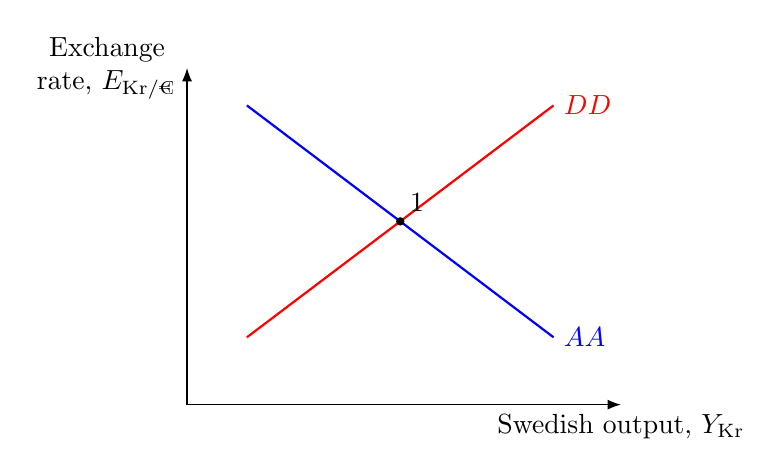
\begin{tikzpicture}[scale=0.95,>=Latex]
\draw[->] (0,0) -- (0,4.5) node[left,align=center]{Exchange\\rate, \(\Ekr\)};
\draw[->] (0,0) -- (5.8,0) node[below]{Swedish output, \(Y_{\text{Kr}}\)};

\draw[thick,red] (0.8,0.9) -- (4.9,4.0) node[right] {\(DD\)};
\draw[thick,blue] (0.8,4.0) -- (4.9,0.9) node[right] {\(AA\)};

\fill (2.85,2.45) circle (1.6pt) node[above right] {1};
\end{tikzpicture}
\end{center}

\item A \textbf{permanent decrease} in the Swedish money supply is contractionary monetary policy. In the short run, prices are fixed, so
\[
\frac{MS_{\text{Kr}}}{P_{\text{SE}}}\downarrow
\quad \Rightarrow \quad
R_{\text{Kr}}\uparrow.
\]
This raises the return on Swedish deposits and causes the krona to appreciate:
\[
\Ekr \downarrow.
\]

Because the change in money supply is permanent, people also expect a stronger krona in the future, so
\[
\Ekre \downarrow.
\]
That strengthens the appreciation effect even more. Therefore, the \(AA\) curve shifts down, and because the policy is permanent it shifts down by more than it would under a temporary contraction. The \(DD\) curve does not shift.

\begin{center}
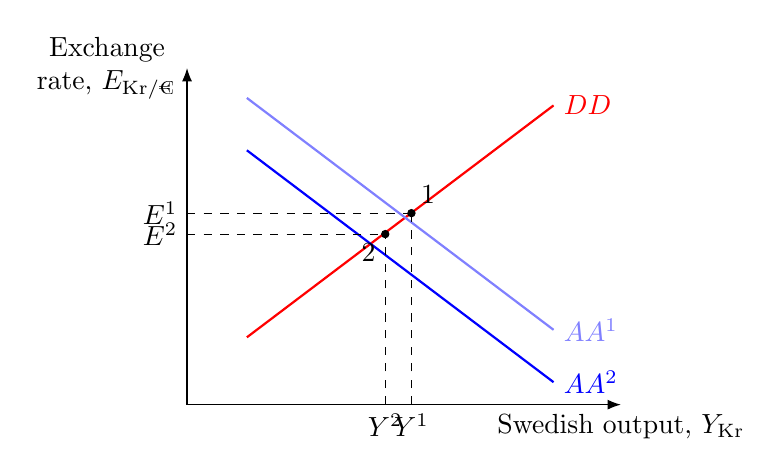
\begin{tikzpicture}[scale=0.95,>=Latex]
\draw[->] (0,0) -- (0,4.5) node[left,align=center]{Exchange\\rate, \(\Ekr\)};
\draw[->] (0,0) -- (5.8,0) node[below]{Swedish output, \(Y_{\text{Kr}}\)};

\draw[thick,red] (0.8,0.9) -- (4.9,4.0) node[right] {\(DD\)};
\draw[thick,blue!50] (0.8,4.1) -- (4.9,1.0) node[right] {\(AA^1\)};
\draw[thick,blue] (0.8,3.4) -- (4.9,0.3) node[right] {\(AA^2\)};

\fill (3.00,2.56) circle (1.6pt) node[above right] {1};
\fill (2.65,2.28) circle (1.6pt) node[below left] {2};

\draw[dashed] (0,2.56) -- (3.00,2.56);
\draw[dashed] (0,2.28) -- (2.65,2.28);
\draw[dashed] (3.00,0) -- (3.00,2.56);
\draw[dashed] (2.65,0) -- (2.65,2.28);

\node[left] at (0,2.56) {\(E^1\)};
\node[left] at (0,2.28) {\(E^2\)};
\node[below] at (3.00,0) {\(Y^1\)};
\node[below] at (2.65,0) {\(Y^2\)};
\end{tikzpicture}
\end{center}

So, in the short run,
\[
Y_{\text{Kr}} \downarrow,
\qquad
\Ekr \downarrow.
\]
Swedish output falls, and the krona appreciates.

\item In the short run, goods prices are assumed to be sticky.

\begin{enumerate}[(i)]
\item The price in kronor of a bag of frozen Swedish meatballs sold in Stockholm is unchanged in the short run. This is exactly the short-run fixed-price assumption.

\item The price in euros of a bag of Swedish meatballs sold in Paris rises. If the Swedish price in Stockholm is fixed in kronor, then the euro price is
\[
P_{\text{\texteuro}}^{\text{Paris}}
=
\frac{P_{\text{Kr}}^{\text{Stockholm}}}{\Ekr}.
\]
Since the krona appreciates, \(\Ekr\) falls. Therefore the denominator falls, so the euro price rises.
\end{enumerate}

\item If the money-supply reduction is temporary instead of permanent, the change in prices from part (c) is:

\begin{enumerate}[(i)]
\item The same for the Stockholm price in kronor: it is still unchanged in the short run.

\item Smaller for the Paris price in euros. The euro price still rises, but it rises by less than in part (c).
\end{enumerate}

\begin{center}
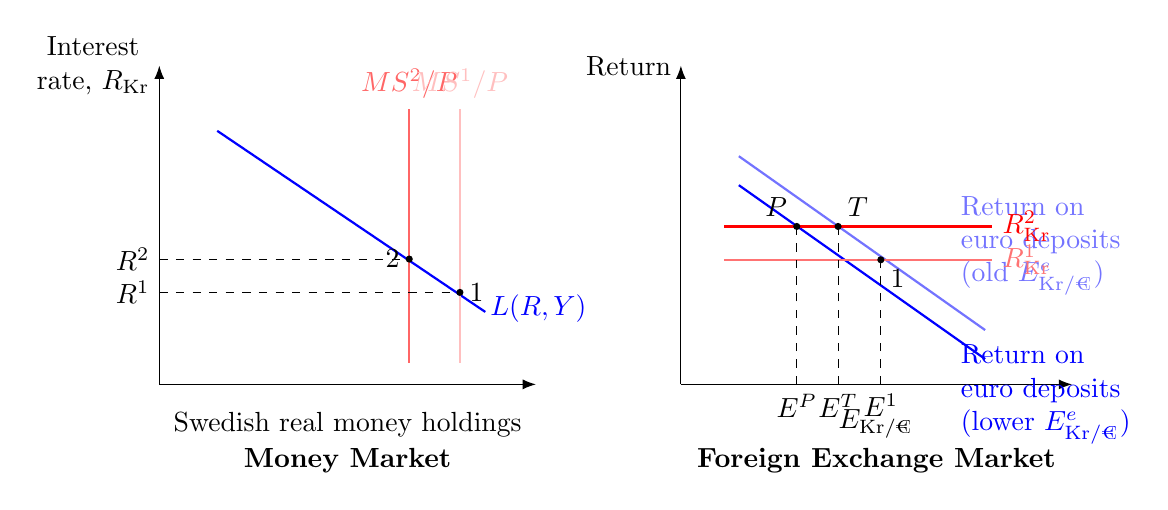
\begin{tikzpicture}[scale=0.92,>=Latex]

%---------------- Left panel: Money market ----------------
\begin{scope}[xshift=0cm]
\draw[->] (0,0) -- (0,4.4) node[left,align=center]{Interest\\rate, $R_{\text{Kr}}$};
\draw[->] (0,0) -- (5.2,0);

% Axis title
\node at (2.6,-0.55) {Swedish real money holdings};

% Money demand
\draw[thick,blue] (0.8,3.5) -- (4.5,1.0)
node[pos=0.98,right] {$L(R,Y)$};

% Money supply lines
\draw[thick,red!60] (3.45,0.3) -- (3.45,3.8)
node[above] {$MS^2/P$};
\draw[thick,red!25] (4.15,0.3) -- (4.15,3.8)
node[above] {$MS^1/P$};

% Equilibrium points
\fill (4.15,1.27) circle (1.4pt) node[right] {$1$};
\fill (3.45,1.73) circle (1.4pt) node[left] {$2$};

% Dashed guides
\draw[dashed] (0,1.27) -- (4.15,1.27);
\draw[dashed] (0,1.73) -- (3.45,1.73);

% Interest-rate labels
\node[left] at (0,1.27) {$R^1$};
\node[left] at (0,1.73) {$R^2$};

% Panel title
\node at (2.6,-1.05) {\textbf{Money Market}};
\end{scope}

%---------------- Right panel: Foreign exchange market ----------------
\begin{scope}[xshift=7.2cm]
\draw[->] (0,0) -- (0,4.4) node[left]{Return};
\draw[->] (0,0) -- (5.4,0);

% Axis title
\node at (2.7,-0.55) {$E_{\text{Kr}/\text{\texteuro}}$};

% Return on euro deposits: old expected future exchange rate
\draw[thick,blue!55] (0.8,3.15) -- (4.2,0.75)
node[pos=0.86,above right,align=left]
{Return on\\euro deposits\\(old $E^e_{\text{Kr}/\text{\texteuro}}$)};

% Return on euro deposits: lower expected future exchange rate
\draw[thick,blue] (0.8,2.75) -- (4.2,0.35)
node[pos=0.86,below right,align=left]
{Return on\\euro deposits\\(lower $E^e_{\text{Kr}/\text{\texteuro}}$)};

% Return on kr deposits
\draw[thick,red!55] (0.6,1.72) -- (4.3,1.72)
node[right] {$R^1_{\text{Kr}}$};
\draw[thick,red] (0.6,2.18) -- (4.3,2.18)
node[right] {$R^2_{\text{Kr}}$};

% Equilibrium points
\fill (2.76,1.72) circle (1.4pt) node[below right] {$1$};
\fill (2.17,2.18) circle (1.4pt) node[above right] {$T$};
\fill (1.60,2.18) circle (1.4pt) node[above left] {$P$};

% Dashed guides
\draw[dashed] (2.76,0) -- (2.76,1.72);
\draw[dashed] (2.17,0) -- (2.17,2.18);
\draw[dashed] (1.60,0) -- (1.60,2.18);

% Exchange-rate labels
\node[below] at (1.60,0) {$E^P$};
\node[below] at (2.17,0) {$E^T$};
\node[below] at (2.76,0) {$E^1$};

% Panel title
\node at (2.7,-1.05) {\textbf{Foreign Exchange Market}};
\end{scope}

\end{tikzpicture}
\end{center}

A temporary decrease in the money supply raises Swedish interest rates, so the return on kronor deposits rises from \(R^1_{\text{Kr}}\) to \(R^2_{\text{Kr}}\). This moves the equilibrium exchange rate from \(E^1\) to \(E^T\), so the krona appreciates.

But a permanent decrease in the money supply does more than that. It also makes people expect a stronger krona in the future, so \(\Ekre\) falls. That shifts the return on euro deposits downward and moves the exchange rate further to \(E^P\). Therefore,
\[
E^P < E^T < E^1.
\]

So the temporary contraction causes a smaller appreciation of the krona than the permanent contraction. Therefore the rise in the Paris euro price is smaller under a temporary decrease in the money supply.

\end{enumerate}

\end{problem}

%--------------------------------------------------
\begin{problem}{2}

\begin{enumerate}[(a)]

\item If people expect the Danish central bank to permanently increase the money supply in the near future, then they will expect higher prices in the future. In the long run, a higher money supply implies a higher domestic price level.

\item Now assume those inflation expectations cause prices to rise today. In the AA-DD model:

\[
P_{\text{DK}}\uparrow
\quad \Rightarrow \quad
\frac{MS_{\text{Kr}}}{P_{\text{DK}}}\downarrow
\quad \Rightarrow \quad
R_{\text{Kr}}\uparrow,
\]
so the \(AA\) curve shifts down.

Also, when Danish prices rise, Danish goods become more expensive relative to foreign goods, so the current account falls. Therefore the \(DD\) curve shifts left.

\begin{center}
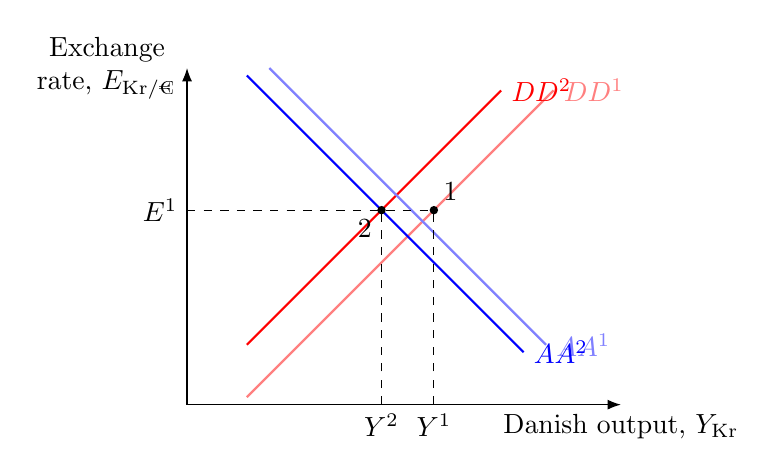
\begin{tikzpicture}[scale=0.95,>=Latex]
\draw[->] (0,0) -- (0,4.5) node[left,align=center]{Exchange\\rate, \(\Ekr\)};
\draw[->] (0,0) -- (5.8,0) node[below]{Danish output, \(Y_{\text{Kr}}\)};

\draw[thick,red!50] (0.8,0.1) -- (4.9,4.2) node[right] {\(DD^1\)};
\draw[thick,red] (0.8,0.8) -- (4.2,4.2) node[right] {\(DD^2\)};

\draw[thick,blue!50] (1.1,4.5) -- (4.8,0.8) node[right] {\(AA^1\)};
\draw[thick,blue] (0.8,4.4) -- (4.5,0.7) node[right] {\(AA^2\)};

\fill (3.30,2.60) circle (1.6pt) node[above right] {1};
\fill (2.60,2.60) circle (1.6pt) node[below left] {2};

\draw[dashed] (0,2.60) -- (3.30,2.60);
\draw[dashed] (2.60,0) -- (2.60,2.60);
\draw[dashed] (3.30,0) -- (3.30,2.60);

\node[left] at (0,2.60) {\(E^1\)};
\node[below] at (2.60,0) {\(Y^2\)};
\node[below] at (3.30,0) {\(Y^1\)};
\end{tikzpicture}
\end{center}

The economy moves from point 1 to point 2. Output falls:
\[
Y_{\text{Kr}}\downarrow.
\]
\[
\Ekr \text{ unchanged}.
\]

\item Since output falls below full employment, the Danish central bank should undertake expansionary monetary policy, meaning it should increase the money supply. That shifts the \(AA\) curve upward, lowers interest rates, and depreciates the krone enough to move the economy back to full employment.

\item Yes, in this setup it is a self-fulfilling prophecy.

The original belief is that the central bank will increase the money supply in the future. That belief causes people to expect higher future prices. Those expectations then raise prices today. The higher current price level reduces real money balances and hurts the current account, which lowers output. Because the central bank has a full-employment mandate, it now has an incentive to increase the money supply to bring output back up. So the original expectation can cause behavior that makes the monetary expansion actually occur.

\end{enumerate}

\end{problem}

\end{document}